\documentclass[t]{beamer}
\listfiles
\usepackage[utf8]{inputenc}
\usepackage[T1]{fontenc}
\usepackage{fontawesome}
\usepackage{ifthen}
\usepackage[overlay,absolute]{textpos}
\usepackage{graphicx}
\graphicspath{{./img/}}
\usepackage{hyperref}

\begin{document}

\begin{frame}[plain,label=titel]
  \begin{textblock}{0}(0.05,2)
    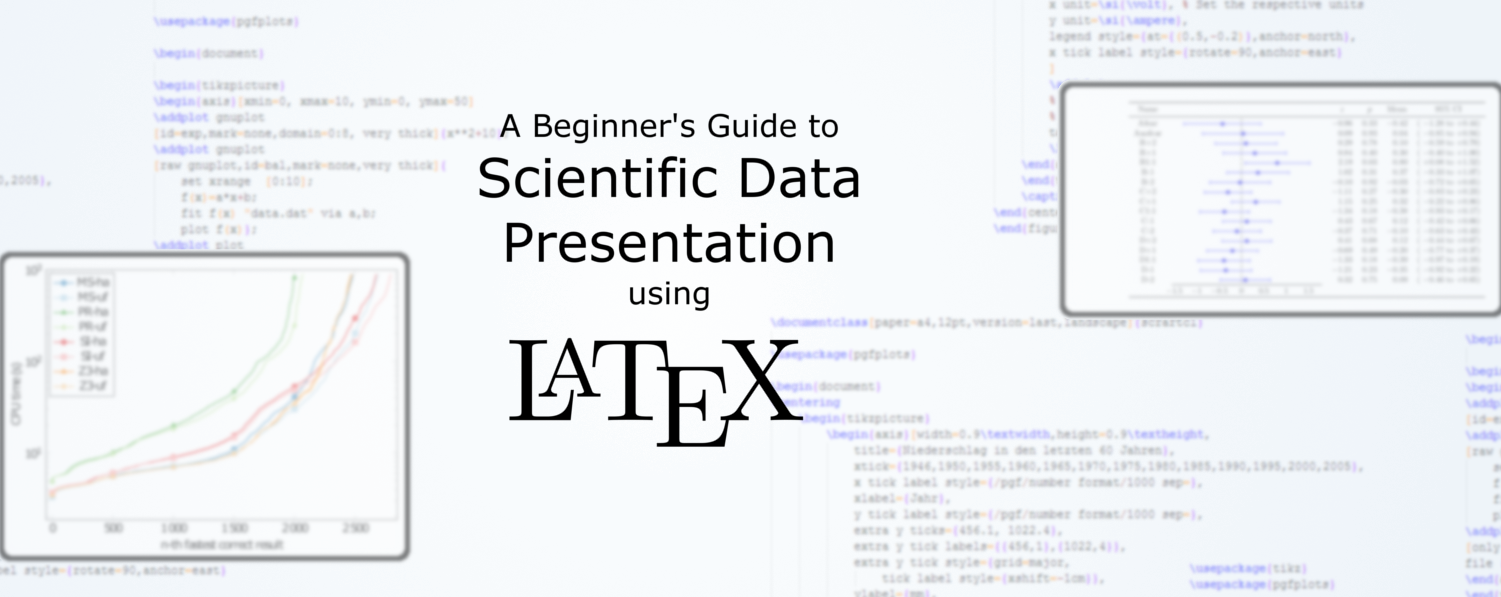
\includegraphics{banner}
  \end{textblock}
  \begin{textblock}{20}(1.5,11)
    \small Stephan Lukasczyk — IEEE Student Branch Passau — 2016--06--16
  \end{textblock}
\end{frame}

\begin{frame}
  \frametitle{Before you fall asleep\dots}
  \begin{textblock}{0}(1,2)
    \onslide<1->{
      
\includegraphics[width=4in]{powerpoint}
    }
  \end{textblock}

  \begin{textblock}{0}(5,5)
    \onslide<2->{
      
\includegraphics[width=3in,angle=350]{death-powerpoint}
    }
  \end{textblock}
\end{frame}

\begin{frame}
  \begin{textblock}{10}(5,7)
    \LARGE Presenting Numbers
  \end{textblock}
\end{frame}

\begin{frame}
  \begin{textblock}{10}(7,7)
    \LARGE Tables
  \end{textblock}
\end{frame}

\begin{frame}
  \begin{textblock}{10}(7,7)
    \LARGE Plots
  \end{textblock}
\end{frame}

\begin{frame}
  \frametitle{Something different}
  \begin{textblock}{0}(0.15,2)
    
\includegraphics[width=4.5cm]{tex-stammtisch}
  \end{textblock}
  \begin{textblock}{6}(8,2)
    Bayerischer \TeX{} Stammtisch, July 30, Regensburg\\
    \href{https://doodle.com/poll/k2dvspqra7pz57hv}{Doodle Poll}
  \end{textblock}

  \begin{textblock}{0}(0.15,9)
    
\includegraphics[width=4.5cm]{tex-workshop}
  \end{textblock}
  \begin{textblock}{6}(8,9)
    \LaTeX{} Beginner's Workshop\\
    \href{https://doodle.com/poll/8v3rhrxe2r4zwm4d}{Doodle Poll}
  \end{textblock}
\end{frame}

\begin{frame}
  \frametitle{Summary}
  \begin{textblock}{0}(0.15,2)
    \onslide<1->{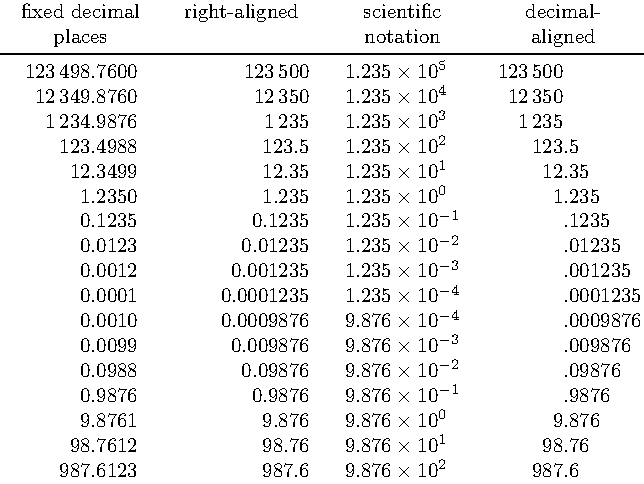
\includegraphics[width=5cm]{numbers}}
  \end{textblock}
  \begin{textblock}{0}(8,2)
    \onslide<2->{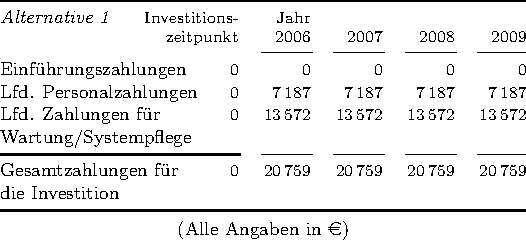
\includegraphics[width=6cm]{table-good}} 
  \end{textblock}

  \begin{textblock}{0}(0.15,9)
    \onslide<3->{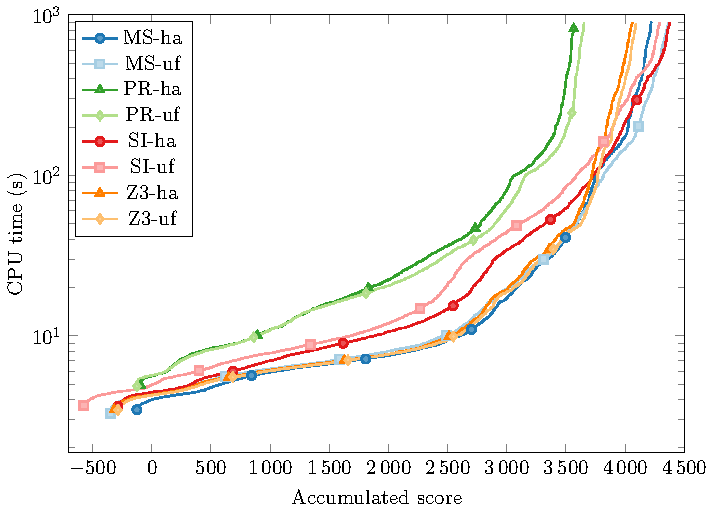
\includegraphics[width=5cm]{quantileplot}}
  \end{textblock}
  \begin{textblock}{6}(8,9)
    \onslide<4->{
    \faGithub~\href{https://github.com/IEEE-SB-Passau/latex-data-presentation}%
      {IEEE-SB-Passau/latex-data-presentation}\\
    \faCode~\href{https://research.lukasczyk.me/latex-data-presentation}%
      {https://research.lukasczyk.me/latex-data-presentation}\\
    \faTwitter~\href{https://twitter.com/erdmaennchen42}{@erdmaennchen42}
    }
  \end{textblock}
\end{frame}

\end{document}
